\documentclass[10pt,twocolumn]{article}
\usepackage[a4paper,margin=0.8in]{geometry}
\usepackage[T1]{fontenc}
\usepackage[utf8]{inputenc}
\usepackage{lmodern}
\usepackage{amsmath,amssymb,amsthm,mathtools}
\usepackage{bm}
\usepackage{graphicx}
\usepackage{booktabs}
\usepackage{microtype}
\usepackage[numbers]{natbib}
\usepackage[colorlinks=true,linkcolor=blue,citecolor=blue,urlcolor=blue]{hyperref}
\usepackage{caption}
\setlength{\columnsep}{0.24in}
\setlength{\parskip}{0.25em}
\setlength{\parindent}{0pt}

\newcommand{\IISCLogo}{
\includegraphics[height=1.45cm]{assets/small_iisc_logo.png}}
\newcommand{\RBCCPSLogo}{
\includegraphics[width=0.95\linewidth,height=1.25cm,keepaspectratio]{assets/small_rbccps_logo_clean.png}}
\begin{document}
\twocolumn[{%
\begin{center}
\begin{minipage}{0.45\textwidth}\raggedright
\IISCLogo
\end{minipage}\hfill
\begin{minipage}{0.45\textwidth}\raggedleft
\RBCCPSLogo
\end{minipage}

\vspace{0.8em}
{\LARGE\bfseries Project Summary\par}
\vspace{0.35em}
{\large Operational Transport Geometry for Representation Learning\par}
\vspace{0.5em}
{RBCCPS, Indian Institute of Science, Bangalore\par}
\vspace{1.0em}
\end{center}
}]

\section{Introduction and Novelty}

Optimal transport provides a principled way to compare probability measures by asking how much it costs to move mass from one distribution to another. In its classical Kantorovich form, a transport distance is determined not only by the two distributions being compared, but also by the ground cost that specifies the cost of matching one point to another. This makes optimal transport especially attractive for representation learning: unlike pointwise losses, it can compare entire distributions while preserving geometric structure. Computational developments such as entropic regularization and scalable solvers have made these ideas usable in modern machine learning settings \citep{peyre_cuturi_computational_ot, cuturi_sinkhorn}.

A large body of work has therefore used optimal transport for domain adaptation. In this view, a source domain and a target domain induce different feature distributions, and the goal is to align these distributions so that a predictor trained on one domain transfers to another. Classical OT-based domain adaptation learns a transport plan between source and target distributions \citep{courty_ot_da}; neural variants such as WDGRL use Wasserstein discrepancy to guide domain-invariant representation learning \citep{shen_wdgrl}; and joint-distribution methods such as DeepJDOT align feature-label structure rather than only marginal feature distributions \citep{deepjdot}. These approaches established that transport can be useful for representation alignment under distribution shift.

However, ordinary domain alignment is often too coarse for deployed systems. A deployed system is rarely a single predictor ending at a label. It is usually a multi-stage computational object: inputs pass through intermediate modules, representations, estimators, controllers, or decision operators before producing the final operational output. In such systems, not every domain shift should be removed. Some variations are nuisance variations and should be collapsed. Some variations are semantically meaningful but operationally harmless. Some variations are operationally consequential and must be preserved. A purely domain-invariant representation may therefore be inappropriate: it can remove information that is irrelevant to labels but essential to downstream operation.

Recent task-aware and invariance-based methods recognize parts of this issue. Task-driven discrepancy measures argue that probability discrepancies should be shaped by downstream predictors rather than treated as task-independent objects \citep{task_driven_discrepancy}. ToAlign studies which feature components should be aligned and which should be ignored for the classification task \citep{toalign}. Invariant risk minimization seeks representations that support invariant predictors across environments \citep{irm}, while split invariant-equivariant representation learning explicitly separates invariant and equivariant factors \citep{sie}. Decision-focused learning and smart predict-then-optimize frameworks similarly emphasize that predictive models should be judged by downstream decision quality rather than only by prediction error \citep{decision_focused_learning, smart_predict_then_optimize}.

The remaining gap is structural. These literatures usually attach task information to a predictor, a discrepancy, or a decision objective, while the deployed system itself remains mathematically shallow: either a source-target alignment problem, a representation-invariance problem, or a predict-then-optimize pipeline. The intermediate computational structure of the deployed system is rarely treated as a finite graph whose internal nodes each carry their own representation spaces, domain-induced distributions, and downstream operational consequences. As a result, there is no explicit node-wise geometry saying which internal representation states may be identified, which substitutions are admissible, and which variations must remain separated because they change terminal behavior. The present framework addresses that missing layer by making terminal operational evaluation induce geometry inside the deployed system, not only a scalar loss at its end.

This project formalizes that principle in a transport-geometric setting. We model a deployed system as a finite directed acyclic graph
\[
\mathcal{G}=(V,E),
\]
where each node $v\in V$ carries a state space $\mathcal{Z}_v$. When a node is representation-producing, $\mathcal{Z}_v$ may be modeled as a representation manifold $\mathcal{M}_v$. A deployment domain $d$ induces, through the graph, a node-wise distribution $\mu_v^d$ over $\mathcal{Z}_v$. A terminal operational evaluation functional $\mathcal{E}_{\mathrm{op}}$ judges the final system output. By intervening on an internal node state and executing the downstream subgraph, this terminal evaluation induces a node-wise operational risk
\[
r_v(z),
\]
which measures the downstream operational consequence of reaching state $z$ at node $v$.

\section{Notation and Preliminaries}

All measurable spaces are assumed to be standard Borel, and whenever a metric structure is required we work over Polish spaces. For a Polish space $(\mathcal{Z},d_{\mathcal{Z}})$, let $\mathcal{P}(\mathcal{Z})$ denote the set of Borel probability measures on $\mathcal{Z}$, and let $\mathcal{P}_p(\mathcal{Z})\subseteq\mathcal{P}(\mathcal{Z})$ denote the set of probability measures with finite $p$-th moment. If $f:\mathcal{Z}\rightarrow\mathcal{Z}'$ is measurable and $\mu\in\mathcal{P}(\mathcal{Z})$, the pushforward measure is denoted by $f_{\#}\mu$, where $f_{\#}\mu(A)=\mu(f^{-1}(A))$ for every Borel set $A\subseteq\mathcal{Z}'$. A deployment domain is a law $P_d\in\mathcal{P}(\mathcal{X})$, indexed by $d\in\mathcal{D}$, over an input space $\mathcal{X}$. The deployed system is represented by a finite directed acyclic graph $\mathcal{G}=(V,E)$. Each node $v\in V$ carries a state space $\mathcal{Z}_v$, and each directed edge $(u,v)\in E$ represents admissible information flow from state $z_u\in\mathcal{Z}_u$ to state $z_v\in\mathcal{Z}_v$. Writing $\operatorname{Pa}(v)=\{u\in V:(u,v)\in E\}$, the node computation is a measurable transition
\[
F_v:\prod_{u\in\operatorname{Pa}(v)}\mathcal{Z}_u\rightarrow\mathcal{Z}_v,
\qquad
z_v=F_v((z_u)_{u\in\operatorname{Pa}(v)}).
\]
If the node is representation-producing, we model $\mathcal{Z}_v$ as, or embed it into, a representation manifold $\mathcal{M}_v$, taken to be a finite-dimensional, second-countable, Hausdorff smooth manifold equipped with its Borel $\sigma$-algebra and, when needed, a metric or geodesic distance $d_{\mathcal{M}_v}$. In applications, $\mathcal{M}_v$ may be accessed through a learned encoder, chart map, or projection rather than specified explicitly. If $\Phi_v:\mathcal{X}\rightarrow\mathcal{Z}_v$ denotes the upstream graph map from inputs to node $v$, then domain $d$ induces the node-wise law
\[
\mu_v^d=\operatorname{Law}(z_v\mid x\sim P_d)=(\Phi_v)_{\#}P_d.
\]
When domain-specific node representations are first realized in spaces $\mathcal{M}_v^{(d)}$, we write
\[
\phi_v^{(d)}:\mathcal{M}_v^{(d)}\rightarrow\widetilde{\mathcal{M}}_v
\]
for a measurable projection or alignment map into a shared node representation space $\widetilde{\mathcal{M}}_v$.

We use the Kantorovich formulation of optimal transport. For $\mu,\nu\in\mathcal{P}(\mathcal{Z})$, a coupling or transport plan is a probability measure $\pi\in\mathcal{P}(\mathcal{Z}\times\mathcal{Z})$ whose marginals are $\mu$ and $\nu$. The set of all such couplings is
\[
\Pi(\mu,\nu)
=
\{\pi\in\mathcal{P}(\mathcal{Z}\times\mathcal{Z}):(\mathrm{pr}_1)_{\#}\pi=\mu,\;(\mathrm{pr}_2)_{\#}\pi=\nu\},
\]
where $\mathrm{pr}_1(z,z')=z$ and $\mathrm{pr}_2(z,z')=z'$. Given a lower semicontinuous nonnegative ground cost $c:\mathcal{Z}\times\mathcal{Z}\rightarrow\mathbb{R}_{+}$, the Kantorovich optimal transport problem is
\[
\mathsf{OT}_c(\mu,\nu)
=
\inf_{\pi\in\Pi(\mu,\nu)}
\int_{\mathcal{Z}\times\mathcal{Z}} c(z,z')\,d\pi(z,z').
\]
This formulation optimizes over transport plans rather than deterministic maps, making it suitable for comparing distributions whose mass may split across multiple target regions. When $c(z,z')=d_{\mathcal{Z}}(z,z')^p$, the corresponding $p$-Wasserstein distance is
\[
W_p(\mu,\nu)
=
\left(
\inf_{\pi\in\Pi(\mu,\nu)}
\int_{\mathcal{Z}\times\mathcal{Z}}d_{\mathcal{Z}}(z,z')^p\,d\pi(z,z')
\right)^{1/p}.
\]
In the present framework, the ordinary metric cost $d_{\mathcal{Z}}^p$ is treated only as a baseline. The relevant transport object will use node-dependent operational costs and, when semantic or operational restrictions are present, a restricted admissible coupling class
\[
\Pi_{\mathrm{adm}}(\mu,\nu)\subseteq\Pi(\mu,\nu).
\]

Let $T\subseteq V$ denote the terminal nodes and let $\mathcal{Y}$ be the terminal output space. The terminal output map is
\[
H:\prod_{t\in T}\mathcal{Z}_t\rightarrow\mathcal{Y},
\qquad
y=H((z_t)_{t\in T}).
\]
Final deployed behavior is evaluated by an operational functional $\mathcal{E}_{\mathrm{op}}:\mathcal{Y}\rightarrow\mathcal{Q}$, or by a scalar operational loss $\mathcal{L}_{\mathrm{op}}:\mathcal{Y}\rightarrow\mathbb{R}_{+}$ when scalarization is appropriate. For an internal node $v$, the intervention $\operatorname{do}(z_v=z)$ fixes the node state to $z$ and executes the downstream subgraph according to the remaining node transitions. A risk functional $\rho$ maps the resulting terminal evaluation or loss to a scalar node-wise risk:
\[
r_v(z)=\rho\left(\mathcal{E}_{\mathrm{op}}(Y)\mid \operatorname{do}(z_v=z)\right),
\]
or, in the scalar-loss case,
\[
r_v(z)=\rho\left(\mathcal{L}_{\mathrm{op}}(Y)\mid \operatorname{do}(z_v=z)\right).
\]
The functional $\rho$ may be expectation, worst-case risk, conditional value-at-risk, or another deployment-appropriate risk measure. These objects fix the notation for the operational geometry constructed in the following section.

\section{Methodology}

We model the deployed system as a finite directed acyclic graph
\[
\mathcal{G}=(V,E),
\]
where each node $v\in V$ carries a state space $\mathcal{Z}_v$. When $v$ is representation-producing, we may impose the more specific regularity assumption
\[
\mathcal{Z}_v=\mathcal{M}_v,
\]
where $\mathcal{M}_v$ is a representation manifold. For a node $v$, the parent set is $\operatorname{Pa}(v)$, and the node computation is represented by
\[
F_v:\prod_{u\in\operatorname{Pa}(v)}\mathcal{Z}_u\rightarrow \mathcal{Z}_v,
\qquad
z_v=F_v((z_u)_{u\in\operatorname{Pa}(v)}).
\]
A deployment domain $d\in\mathcal{D}$ is a law $P_d\in\mathcal{P}(\mathcal{X})$. Passing $P_d$ through the graph induces a node-wise distribution
\[
\mu_v^d=\operatorname{Law}(z_v\mid x\sim P_d).
\]
Equivalently, if $\Phi_v:\mathcal{X}\rightarrow\mathcal{Z}_v$ is the upstream graph map from input to node $v$, then
\[
\mu_v^d=(\Phi_v)_{\#}P_d.
\]
In the manifold case, $\Phi_v:\mathcal{X}\rightarrow\mathcal{M}_v$ and $\mu_v^d\in\mathcal{P}(\mathcal{M}_v)$.

Let $T\subseteq V$ be the set of terminal nodes. The final system output is
\[
y=H((z_t)_{t\in T}).
\]
At the most general level, final behavior is judged by an operational evaluation functional
\[
\mathcal{E}_{\mathrm{op}}:\mathcal{Y}\rightarrow\mathcal{Q}.
\]
As a scalar-loss instantiation, one may use
\[
\mathcal{L}_{\mathrm{op}}:\mathcal{Y}\rightarrow\mathbb{R}_{+},
\]
or, when targets, contexts, or constraints are available,
\[
\mathcal{L}_{\mathrm{op}}:\mathcal{Y}\times\mathcal{Y}_{\mathrm{target}}\times\mathcal{C}\rightarrow\mathbb{R}_{+}.
\]
For an internal node $v$, the intervention $\operatorname{do}(z_v=z)$ fixes the node state to $z$ and executes the downstream subgraph. This induces a node-wise operational risk
\[
r_v(z)=\rho\left(\mathcal{E}_{\mathrm{op}}(Y)\mid\operatorname{do}(z_v=z)\right),
\]
or, in the scalar-loss case,
\[
r_v(z)=\rho\left(\mathcal{L}_{\mathrm{op}}(Y)\mid\operatorname{do}(z_v=z)\right).
\]
The risk functional $\rho$ may be expectation, worst-case risk, conditional value-at-risk, or another deployment-appropriate risk measure.

Low-risk and high-risk regions are abstractly defined by an acceptability rule on node states. A threshold-level-set instantiation is
\[
\mathcal{A}_v(\tau)=\{z\in\mathcal{Z}_v:r_v(z)\leq \tau\},
\qquad
\mathcal{B}_v(\kappa)=\{z\in\mathcal{Z}_v:r_v(z)\geq \kappa\}.
\]
In the manifold case, replace $\mathcal{Z}_v$ by $\mathcal{M}_v$. Here $\tau$ is an acceptability threshold and $\kappa$ is a failure threshold.

Semantic compatibility is represented abstractly by a node-wise relation
\[
z\sim_{\mathrm{sem},v}z'.
\]
A descriptor-based instantiation introduces
\[
s_v:\mathcal{Z}_v\rightarrow\mathcal{S}_v
\]
and declares compatibility when
\[
d_{\mathrm{sem}}(s_v(z),s_v(z'))\leq \varepsilon_{\mathrm{sem}}.
\]
Let $G_v:\mathcal{Z}_v\rightarrow\mathcal{Y}$ denote the downstream map from node $v$ to the final output. One possible operational discrepancy is
\[
\Delta_v(z,z')
=
d_{\mathcal{Y}}(G_v(z),G_v(z'))
+
|r_v(z)-r_v(z')|.
\]

The tilted operational geometry is defined by a node-wise ground cost
\[
c_v:\mathcal{Z}_v\times\mathcal{Z}_v\rightarrow\mathbb{R}_{+}.
\]
In the manifold case,
\[
c_v:\mathcal{M}_v\times\mathcal{M}_v\rightarrow\mathbb{R}_{+}.
\]
A concrete weighted construction is
\[
\begin{aligned}
c_v(z,z')
=&\;\alpha d_{\mathcal{M}_v}(z,z')^p
+\beta d_{\mathrm{sem}}(s_v(z),s_v(z'))^p\\
&+\gamma |r_v(z)-r_v(z')|^p
+\eta d_{\mathcal{Y}}(G_v(z),G_v(z'))^p
+\lambda \mathbf{1}_{\mathrm{incompat}}(z,z').
\end{aligned}
\]
This expression is only one instantiation. The general object is the cost $c_v$, which equips the node state space with an operational-semantic geometry.

For two domains $d,d'$, the ordinary Wasserstein comparison is replaced by a node-wise operational transport distance using $c_v$ and an admissible coupling class:
\[
W_{v,\mathrm{op}}(\mu_v^d,\mu_v^{d'})^p
=
\inf_{\pi\in\Pi_{\mathrm{adm}}(\mu_v^d,\mu_v^{d'})}
\int_{\mathcal{Z}_v\times\mathcal{Z}_v}c_v(z,z')\,d\pi(z,z').
\]
The admissible coupling set $\Pi_{\mathrm{adm}}$ restricts mass transport to semantically compatible or operationally substitutable states. If full mass matching is inappropriate, one may instead use an unbalanced version:
\[
UW_{v,\mathrm{op}}(\mu,\nu)^p
=
\inf_{\pi\geq 0}
\left[
\int c_v(z,z')\,d\pi(z,z')
+\rho_1D(\pi_1\Vert\mu)
+\rho_2D(\pi_2\Vert\nu)
\right],
\]
where $\pi_1,\pi_2$ are the marginals of $\pi$, and the divergence terms penalize unmatched or reweighted mass.

A full system-level discrepancy is obtained by aggregating node-wise operational transport distances:
\[
D_{\mathrm{op}}(d,d')
=
\mathfrak{A}\left(\{W_{v,\mathrm{op}}(\mu_v^d,\mu_v^{d'})\}_{v\in V}\right).
\]
A weighted-sum instantiation is
\[
D_{\mathrm{op}}(d,d')
=
\sum_{v\in V}\omega_v W_{v,\mathrm{op}}(\mu_v^d,\mu_v^{d'})^p.
\]
If the goal is movement toward operational safety rather than domain-to-domain alignment, one may define a safe target law $Q_v$ with
\[
\operatorname{supp}(Q_v)\subseteq \mathcal{A}_v(\tau)
\]
and optimize, for learnable objects $\Theta$,
\[
\min_{\Theta}
\sum_{d\in\mathcal{D}}
\sum_{v\in V}
\omega_v W_{v,\mathrm{op}}(\mu_{v,\Theta}^d,Q_v)^p
+
\mathcal{R}(\Theta).
\]
Here $\Theta$ may include projection maps, manifold coordinates, risk estimators, semantic descriptors, cost parameters, or safe target distributions, while $\mathcal{R}(\Theta)$ prevents collapse and preserves downstream-relevant information.

The resulting flow is
\[
\mathcal{G}=(V,E)
\Rightarrow
\{\mathcal{Z}_v\}_{v\in V}
\Rightarrow
\{\mu_v^d\}_{v\in V,d\in\mathcal{D}}
\Rightarrow
\mathcal{E}_{\mathrm{op}}
\Rightarrow
\{r_v\}_{v\in V},
\]
followed by
\[
\{r_v\}_{v\in V}
\Rightarrow
\{\mathcal{A}_v,\mathcal{B}_v\}_{v\in V}
\Rightarrow
\{c_v,\Pi_{\mathrm{adm}}\}_{v\in V}
\Rightarrow
\{W_{v,\mathrm{op}}\}_{v\in V}
\Rightarrow
D_{\mathrm{op}}.
\]
In the manifold-specific version, the state spaces $\mathcal{Z}_v$ are replaced by representation manifolds $\mathcal{M}_v$. Thus domains induce distributions on node state spaces or node manifolds; terminal operational evaluation induces node-wise risk; node-wise risk defines operational regions; semantic compatibility and operational consequence define the tilted ground cost and admissible coupling class; and constrained or unbalanced transport compares domain-induced node distributions under this operational geometry.

\section{Research Questions}

At theorem level, the central question is whether operational consequence can induce a valid geometry on representation distributions. More precisely, we ask under what assumptions a node-wise operational ground cost
\[
c_v:\mathcal{Z}_v\times\mathcal{Z}_v\rightarrow\mathbb{R}_{+}
\]
defines a pseudo-metric, transport divergence, or Wasserstein-type distance on domain-induced representation laws, such that the zero-distance equivalence classes correspond exactly to transformations that preserve downstream operational behavior.

We instantiate this question in a streetlight-object detection and measurement system. In streetlight auditing, the upstream predictor detects, localizes, or represents streetlight structures, while the downstream operator estimates useful illumination, coverage, adequacy, glare, or other operational quantities required for an audit report. Deployment shifts such as glare, scale, viewpoint, blur, occlusion, road geometry, compression, and sensor quality should not be treated as equivalent sources of domain shift. Some shifts are operationally harmless and should be absorbed by the representation. Others change the final illumination report and must be preserved, calibrated, or explicitly penalized. The framework asks which shifts may be identified inside representation space and which shifts must remain distinguishable because they alter downstream operational risk.

The project is organized around the following research questions:
\begin{enumerate}
    \item How should an operational-risk-induced geometry be defined on a node representation space?
    \item How can the node-wise risk $r_v(z)$ be estimated from downstream operational behavior?
    \item How should the low-risk admissible set $\mathcal{A}_v(\tau)$ and high-risk region $\mathcal{B}_v(\kappa)$ be defined?
    \item How can a safe target law $Q_v$ be defined without reducing it to low-loss training examples?
    \item How should $c_v(z,z')$ combine geometric, semantic, and operational discrepancy beyond a weighted Euclidean loss?
    \item When does $c_v$ induce a pseudo-metric or transport distance on representation distributions?
\end{enumerate}

\section{Expected Outputs and Use Cases}

The main expected output is a mathematical project paper defining operational transport geometry for representation learning under deployment shift. The paper should include the graph-based formalism, the node-wise risk construction, the operational ground cost, admissible coupling classes, constrained and unbalanced transport variants, and system-level aggregation. A complete version should also characterize conditions under which the proposed object is a pseudo-metric or transport divergence, identify the induced zero-distance equivalence relation, and state when operationally consequential variations cannot be collapsed without positive cost or inadmissibility.

A second expected output is an applied instantiation for streetlight auditing. This should define the relevant node representations, downstream operational report, risk estimator, low-risk set, semantic compatibility relation, and operational transport cost for a detection-to-measurement pipeline. In this setting, the framework can be used to diagnose whether shifts such as glare, occlusion, scale, viewpoint, blur, compression, and sensor variation affect the final illumination or adequacy report. The intended result is selective operational invariance: collapse what is harmless, preserve what changes the audit.

Mathematical use cases include defining quotient geometries on representation spaces, comparing probability measures under downstream-risk-induced costs, constructing admissible transport problems with semantic constraints, studying stability of representation distributions under operational perturbations, and characterizing when a learned representation preserves terminal behavior. Machine learning use cases include domain adaptation under operational constraints, robust representation learning for deployed perception systems, calibration-aware feature alignment, safety-directed latent transport, and task-aware distribution matching where the task is not merely classification accuracy but final system-level adequacy.

\section{Project Team}

This project is being developed at the Robert Bosch Centre for Cyber-Physical Systems (RBCCPS), Indian Institute of Science, Bangalore. The project team consists of
\[
\begin{array}{ll}
\text{Angad Singh Ahuja} & \text{RBCCPS, IISc Bangalore} \\
\text{Arindam Bhaduri} & \text{RBCCPS, IISc Bangalore} \\
\text{Prof. Prasant Misra} & \text{RBCCPS, IISc Bangalore} \\
\text{Dr. Pandrasamy Arjunan} & \text{RBCCPS, IISc Bangalore}
\end{array}
\]

\begin{thebibliography}{99}

\bibitem{peyre_cuturi_computational_ot}
Gabriel Peyr\'e and Marco Cuturi.
\newblock \emph{Computational Optimal Transport}.
\newblock Foundations and Trends in Machine Learning, 2019.

\bibitem{cuturi_sinkhorn}
Marco Cuturi.
\newblock Sinkhorn distances: Lightspeed computation of optimal transport.
\newblock In \emph{Advances in Neural Information Processing Systems}, 2013.

\bibitem{courty_ot_da}
Nicolas Courty, R\'emi Flamary, Devis Tuia, and Alain Rakotomamonjy.
\newblock Optimal transport for domain adaptation.
\newblock \emph{IEEE Transactions on Pattern Analysis and Machine Intelligence}, 2017.

\bibitem{shen_wdgrl}
Judy Hoffman Shen et al.
\newblock Wasserstein distance guided representation learning for domain adaptation.
\newblock In \emph{AAAI}, 2018.

\bibitem{deepjdot}
Bharath Bhushan Damodaran, Benjamin Kellenberger, R\'emi Flamary, Devis Tuia, and Nicolas Courty.
\newblock DeepJDOT: Deep joint distribution optimal transport for unsupervised domain adaptation.
\newblock In \emph{ECCV}, 2018.

\bibitem{task_driven_discrepancy}
Mikhail Yurochkin, Yuekai Sun, and others.
\newblock Task-driven optimal transport.
\newblock Preprint / task-aware discrepancy line of work.

\bibitem{toalign}
ToAlign authors.
\newblock ToAlign: Task-oriented alignment for domain adaptation.
\newblock Relevant recent task-aware alignment work.

\bibitem{irm}
Martin Arjovsky, L\'eon Bottou, Ishaan Gulrajani, and David Lopez-Paz.
\newblock Invariant risk minimization.
\newblock Preprint, 2019.

\bibitem{sie}
Representative split invariant-equivariant representation learning work.
\newblock Split invariant-equivariant representation learning.
\newblock Relevant invariance literature.

\bibitem{decision_focused_learning}
Brandon Amos and J. Zico Kolter.
\newblock OptNet / decision-focused learning line of work.
\newblock Relevant downstream-decision literature.

\bibitem{smart_predict_then_optimize}
Justin Elmachtoub and Paul Grigas.
\newblock Smart predict-then-optimize.
\newblock \emph{Management Science}, 2022.

\end{thebibliography}

\clearpage
\onecolumn
\thispagestyle{plain}
\begin{center}
\vspace*{\fill}
\makebox[\textwidth][c]{%
\rotatebox[origin=c]{90}{%
\begin{minipage}{0.78\textheight}
\centering
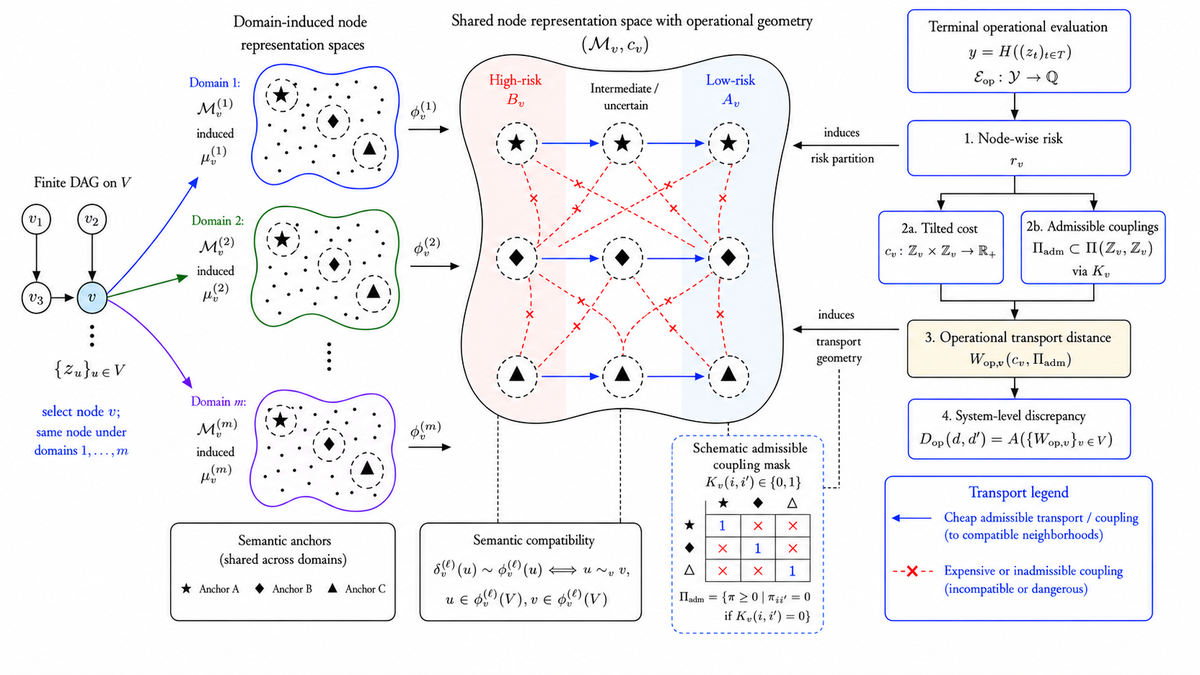
\includegraphics[width=\linewidth]{assets/small_framework_diagram.png}
\captionof{figure}{Schematic overview of the proposed framework. A finite computational DAG induces domain-specific node representations, which are aligned through projections into a shared node representation space equipped with operational geometry. Terminal operational evaluation induces node-wise risk, which shapes both the admissible coupling structure and the operational transport geometry used to compare or adapt domain-induced node distributions.}
\label{fig:framework}
\end{minipage}}}
\vspace*{\fill}
\end{center}

\end{document}
